\subsection{Timecode interface}

\begin{figure}[ht]
  \begin{center}
    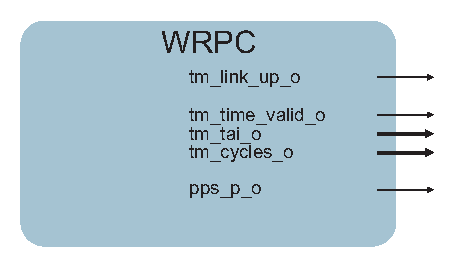
\includegraphics[width=.5\textwidth]{fig/basic_wrpc_tm.pdf}
    \caption{Timecode output interface of WRPC}
  \end{center}
\end{figure}

Timecode interface provides current time to the other HDL modules in a form that
can be easily used. It consists of: a 1-PPS and a UTC timecode
aligned to the time of WR Master.
\begin{center}
  \begin{tabular}{|l|l|p{10cm}|}
    \hline
    {\bf Signal name} & {\bf size} & {\bf description} \\
    \hline \hline
    \texttt{tm\_link\_up\_o} & 1 & state of Ethernet link (up/down), \emph{1}
    means Ethernet link is up\\
    \texttt{tm\_time\_valid\_o} & 1 & if \emph{1}, the timecode generated by the
    WRPC is valid\\
    \texttt{tm\_tai\_o} & 40 & TAI part of the timecode (full seconds)\\
    \texttt{tm\_cycles\_o} & 28 & fractional part of each second represented by
    the state of counter clocked with the frequency 125 MHz (values from 0 to
    124999999, each count is 8 ns)\\
    \texttt{pps\_p\_o} & 1 & 1-PPS signal generated in \emph{clk\_ref\_i} clock
    domain and aligned to WR time, pulse
    generated when the cycle counter is 0 (beginning of each full TAI second)\\
    \hline
  \end{tabular}
\end{center}
